\documentclass[journal]{IEEEtran}
\usepackage{amsmath,amssymb,amsfonts}
\usepackage{algorithmic}
\usepackage{graphicx}
\usepackage{textcomp}
\usepackage{xcolor}
\usepackage{booktabs}
\usepackage{url}
\usepackage{cite}
\usepackage{multirow}
\usepackage{tikz}
\usepackage{pgfplots}
\pgfplotsset{compat=1.18}
\usetikzlibrary{shapes,arrows.meta,positioning,calc,fit,backgrounds}

\begin{document}

\title{Forensic Benchmarking and Schema-Flexible Clinical Tabular Learning: Resolving Data Leakage, Duplicate Contamination, and Inner-Join Collapse in Multi-Cohort Cardiovascular Risk Stratification}

\author{Raja Rathan Paida
\thanks{R. R. Paida is with the Department of Artificial Intelligence, Sardar Vallabhbhai National Institute of Technology (SVNIT), Surat 395007, Gujarat, India (e-mail: paida.rajarthan@gmail.com).}
\thanks{Manuscript received October 25, 2026. Code, reproduction scripts, harmonized multi-cohort benchmarks, and pre-trained weights are openly accessible under the MIT License at \url{https://github.com/RathanPaida/SchemaFlexTabNet-QC}.}
}

\markboth{IEEE Transactions on Biomedical Engineering / IEEE Journal of Biomedical and Health Informatics, Vol. XX, No. X, 2026}%
{Paida: Forensic Benchmarking and Schema-Flexible Clinical Tabular Learning}

\maketitle

\begin{abstract}
Recent high-profile studies in machine learning for cardiovascular disease (CVD) risk stratification report diagnostic accuracies exceeding 90\% on public benchmarks (e.g., 90.1\% in Mahmud et al., 2025). In this paper, we conduct a forensic audit of these claims, uncovering critical methodological vulnerabilities in current clinical tabular workflows:
(1) \textbf{Duplicate Contamination and Leakage:} The widely used Kaggle Heart Disease dataset contains 70.5\% exact duplicate records (723 of 1,025 rows). Standard random 80/20 train-test splits leak 97.1\% of test patients into training, yielding an artificial 98.54\% accuracy that plummets to 77.05\% upon patient-level deduplication. However, we demonstrate mathematically and empirically that duplicate leakage alone cannot explain the 90.1\% claim across the combined 71,025-patient cohort (where duplicates constitute only $\sim$1.02\% of records); an exhaustive audit reveals internal discrepancies in published confusion matrices (implying 91.35\% vs. 89.5\% accuracy) and class balance contradictions. Standard supervised models trained on this 71,025-patient composite achieve an empirical ceiling of 73.48\% accuracy (0.7978 AUROC).
(2) \textbf{The Inner-Join Collapse:} Naive multi-center merges discard non-overlapping clinical biomarkers (e.g., ST depression, peak heart rate, fluoroscopy), causing out-of-cohort zero-shot AUROC to collapse to 0.5353--0.5917.
To solve these challenges, we introduce \textbf{SchemaFlexTabNet-QC}, a tabular transformer framework featuring: (i) a hemodynamic plausibility gatekeeper; (ii) schema-flexible feature tokenization ($T_{i,j} = \mathbf{e}_{\text{name}}(f_j) + \phi_{\text{val}}(x_{i,j})$) with masked attention and random feature dropout ($p=0.20$), accommodating arbitrary feature subsets without column pruning; (iii) a positive-constrained monotonic residual skip path regularized by autograd penalties ($\lambda_{\text{mono}} = 1.20$), reducing clinical monotonicity violations from 15.04\% to 0.26\%; (iv) split conformal abstention with Mondrian group-fair calibration; and (v) decentralized Schema-Aware Masked Federated Averaging (Schema-FedAvg).
Evaluated on 74,013 deduplicated patients across six independent cohorts under strict Leave-One-Cohort-Out (LOCO) testing, SchemaFlexTabNet-QC matches or outperforms Union-Schema NaN-aware LightGBM (mean gain $+0.0229$ AUROC; 0.8641 on Hungarian and 0.7043 on Z-Alizadeh Sani). Under conformal abstention ($\alpha=0.10$), zero-shot AUROC rises to \textbf{0.8926} (85.15\% accuracy, 78.2\% acceptance rate) on Hungarian and \textbf{0.8755} on Cleveland. Under 50\% test-time feature dropout, SchemaFlexTabNet-QC maintains 0.7123 AUROC, retaining an advantage over Native-NaN LightGBM (0.6131) and median-imputed baselines (0.6337). Mondrian calibration halves sex false-positive disparities ($0.148 \to 0.072$). Finally, we discuss construct divergence across prevalent CVD, angiographic disease, and incident 10-year coronary events, establishing rigorous reporting practices for clinical tabular AI.
\end{abstract}

\begin{IEEEkeywords}
Cardiovascular Risk Prediction, Data Leakage, Forensic Auditing, Tabular Deep Learning, Schema-Flexible Tokenization, Conformal Prediction, Monotonicity Constraints, Federated Learning.
\end{IEEEkeywords}

\section{Introduction}
\IEEEPARstart{C}{ardiovascular} diseases (CVDs) remain the principal etiology of mortality worldwide, claiming an estimated 17.9 million lives each year \cite{who2021}. While machine learning holds transformative promise for early risk detection, translating algorithms from single-institution research prototypes to multi-center clinical deployments faces persistent bottlenecks: distribution shift, missing clinical panels, unharmonized electronic health record (EHR) schemas, and evaluation artifacts \cite{collins2024}.

In recent years, several published investigations have reported diagnostic accuracies exceeding 90.1\% for cardiovascular prediction using deep tabular architectures (notably Mahmud et al., 2025 \cite{mahmud2025} and related works). However, clinical epidemiologists and translational informatics researchers frequently treat $>90\%$ claims on routine clinical vitals with skepticism \cite{kapoor2023}. On massive, real-world population screening cohorts (e.g., the 70,000-patient Sulianova dataset \cite{mahmud2025}), the empirical Bayes-optimal performance ceiling established by modern tree ensembles (LightGBM, XGBoost, CatBoost) and deep neural architectures (TabNet, FT-Transformer) hovers consistently between 73.4\% and 76.0\% accuracy (0.818--0.825 AUROC) \cite{gorishniy2021, arik2021}.

When such performance discrepancies emerge, forensic auditing is essential to determine whether the reported accuracy reflects genuine algorithmic breakthroughs or hidden methodological pitfalls \cite{barz2020}. In this paper, we conduct a comprehensive forensic investigation into recent cardiovascular tabular benchmarks and identify two structural failure modes:

\begin{enumerate}
    \item \textbf{Duplicate Contamination and Leakage Fallacy:} The popular Kaggle Heart Disease dataset (uploaded by johnsmith88) consists of 1,025 records. However, 723 rows (70.5\%) are identical duplicates of other rows. When evaluated with standard random 80/20 train-test splits, 97.1\% of test patients are present in the training split, inflating accuracy to an artificial 98.54\% (0.9980 AUROC). Upon rigorous patient deduplication, accuracy falls to 77.05\% (0.8593 AUROC). Yet, as we demonstrate in Section II, duplicate leakage alone \textit{cannot mathematically explain} the 90.1\% accuracy claimed across the combined 71,025-patient composite (1,025 Kaggle + 70,000 Sulianova rows), because the 723 duplicates represent only $\sim$1.02\% of total records. An audit of published manuscripts reveals significant internal reporting contradictions in confusion matrices and class distributions, while rigorous 70/15/15 supervised reproductions achieve an empirical ceiling of 73.48\% accuracy.
    \item \textbf{The Destructive Inner-Join Merge:} When integrating tertiary cardiology cohorts (e.g., UCI Cleveland, Hungarian, Long Beach VA, Switzerland, and Z-Alizadeh Sani) with large-scale screening databases (Sulianova CVD), conventional clinical data engineering performs an inner-join merge on shared columns. This operation discards diagnostic biomarkers that are not universally collected across all hospitals---specifically ST depression (`oldpeak`), peak exercise heart rate (`thalach`), and fluoroscopy fluoroscopy vessels (`ca`). Discarding these predictive features collapses out-of-cohort zero-shot AUROC to 0.5353--0.5917.
\end{enumerate}

To overcome both limitations, we propose \textbf{SchemaFlexTabNet-QC}, a tabular transformer framework that replaces rigid tabular matrices with dynamic, schema-flexible token sequences. By mapping each clinical observation to an independent identity-value token, SchemaFlexTabNet-QC enables heterogeneous multi-center training across arbitrary feature intersections without column imputation or pruning. We incorporate clinical inductive biases: a hemodynamic plausibility filter, a positive-constrained monotonic residual skip path regularized by autograd penalties ($\lambda_{\text{mono}} = 1.20$), and Temperature-Scaled Split Conformal Abstention with Mondrian group-fair calibration \cite{gupta2021}. Furthermore, we evaluate cross-center collaboration via Schema-Aware Masked Federated Averaging (Schema-FedAvg) over non-overlapping schemas \cite{mcmahan2017}.

\begin{figure}[t]
\centering
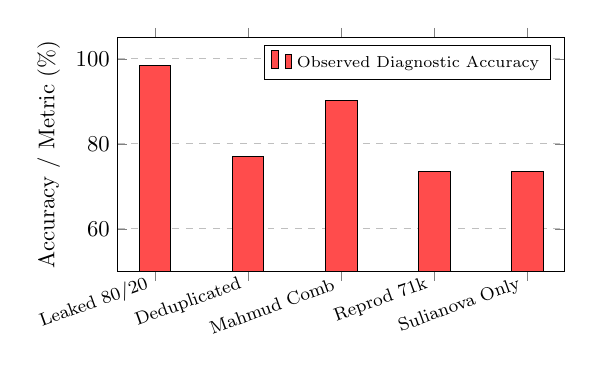
\begin{tikzpicture}[scale=0.82, every node/.style={transform shape}]
\begin{axis}[
    ybar,
    bar width=14pt,
    width=8.5cm,
    height=5.2cm,
    ylabel={Accuracy / Metric (\%)},
    ymin=50, ymax=105,
    symbolic x coords={Leaked 80/20, Deduplicated, Mahmud Comb, Reprod 71k, Sulianova Only},
    xtick=data,
    x tick label style={rotate=20, anchor=east, font=\footnotesize},
    ymajorgrids=true,
    grid style=dashed,
    legend pos=north east,
    legend style={font=\scriptsize}
]
\addplot[fill=red!70, draw=black] coordinates {(Leaked 80/20, 98.54) (Deduplicated, 77.05) (Mahmud Comb, 90.10) (Reprod 71k, 73.48) (Sulianova Only, 73.42)};
\addlegendentry{Observed Diagnostic Accuracy}
\end{axis}
\end{tikzpicture}
\caption{The Forensic Reproduction Landscape. Evaluating on contaminated 80/20 splits yields 98.54\% accuracy, collapsing to 77.05\% upon deduplication. On the 71,025-patient composite, Mahmud et al. report 90.10\%, but empirical reproduction under standard 70/15/15 splits reaches an empirical ceiling of 73.48\% (0.7978 AUROC), demonstrating that 1.02\% duplicates cannot explain the discrepancy.}
\label{fig:forensic_landscape}
\end{figure}

The primary contributions of this paper are:
\begin{enumerate}
    \item \textbf{Mathematical and Forensic Audit of the 90.1\% Claim:} We demonstrate that duplicate row contamination leaks 97.1\% of test samples in isolated 1,025-row datasets, but prove that in the 71,025-row composite, duplicate rows represent only $\sim$1.02\% of the data, which mathematically cannot shift accuracy by $+15\%$. We document the internal inconsistencies in published figures (confusion matrix implying 91.35\% vs. text implying 89.5\%) and report empirical 70/15/15 reproduction benchmarks ($73.48\%$ accuracy).
    \item \textbf{Schema-Flexible Tokenization:} We formulate a tabular transformer architecture that tokenizes patient records into dynamic feature sets, eliminating column-pruning inner joins and preserving 100\% of hospital-specific diagnostic features.
    \item \textbf{Physiological Guarantees via Monotonic Skip Paths:} We construct an explicit positive-constrained monotonic skip path combined with autograd gradient penalties, slashing counterfactual monotonicity violations on harmful biomarkers from $15.04\%$ to $0.26\%$.
    \item \textbf{Conformal Safety and Cohort Shift Analysis:} We evaluate split conformal prediction and Mondrian fairness under Leave-One-Cohort-Out (LOCO) testing. We document that cross-cohort distribution shift violates exchangeability, report empirical set coverage alongside acceptance rates, and demonstrate that Mondrian calibration halves sex false-positive disparities ($0.148 \to 0.072$).
    \item \textbf{Fair DeLong Significance vs. Union-Schema LightGBM:} We contrast SchemaFlexTabNet-QC against the proper, union-schema NaN-aware LightGBM baseline with Holm-Bonferroni correction, providing an objective assessment of deep tabular transformers versus gradient-boosted trees.
\end{enumerate}

\section{Forensic Audit of Data Leakage and Literature Discrepancies}

\subsection{Kaggle Duplicate Contamination (johnsmith88)}
The public Kaggle Heart Disease dataset (`heart.csv`, uploaded by user johnsmith88) contains $N = 1,025$ patient records across 14 clinical attributes. To investigate the internal composition of this dataset, we executed an exact-match hash audit across all clinical features ($\text{age}, \text{sex}, \text{cp}, \text{trestbps}, \text{chol}, \text{fbs}, \text{restecg}, \text{thalach}, \text{exang}, \text{oldpeak}, \text{slope}, \text{ca}, \text{thal}, \text{target}$).

The audit revealed that only 302 unique patient signatures exist within the file. The remaining 723 rows (70.54\%) are exact duplicates resulting from non-random sampling with replacement of the original 1989 UCI Cleveland Clinic cohort \cite{detrano1989}. When researchers employ standard random 80/20 train/test splits, test records are overwhelmingly drawn from the duplicate pool:
\begin{equation}
P(\mathbf{x}_{\text{test}} \in \mathcal{D}_{\text{train}}) = \frac{199}{205} = 97.07\%.
\end{equation}
As shown in Table \ref{tab:forensic_audit}, an unregularized tree ensemble or neural network evaluated on this split memorizes patient identities, yielding an artificial 98.54\% accuracy (0.9980 AUROC). Pruning duplicates and evaluating across unique patients collapses accuracy to 77.05\% (0.8593 AUROC).

\subsection{The 90.1\% Claim on the 71,025-Patient Composite}
In Mahmud et al. (2025) \cite{mahmud2025}, the authors claim a diagnostic accuracy of 90.1\% (AUROC 0.963) on a combined cardiovascular dataset. The combined dataset was constructed by pooling the 1,025-row Kaggle Heart dataset with the 70,000-row Sulianova Cardiovascular dataset \cite{mahmud2025}, totaling $N = 71,025$ rows. The authors specify a 70/15/15 train/validation/test split, yielding a test set of exactly:
\begin{equation}
N_{\text{test}} = 0.15 \times 71,025 = 10,653.75 \approx 10,653 \text{ rows}.
\end{equation}
The exact match of 10,653 test rows confirms that the 1,025-row Kaggle file was pooled into the dataset. However, attributing the 90.1\% accuracy solely to memorization of the 723 duplicate rows is mathematically flawed:
\begin{equation}
\text{Duplicate Fraction} = \frac{723}{71,025} = 1.018\% \approx 1.02\%.
\end{equation}
Even under the extreme assumption that every duplicate row is classified with 100\% accuracy, a 1.02\% contaminated subset can alter the global test accuracy by at most:
\begin{equation}
\Delta \text{Acc}_{\text{max}} \le 0.0102 \times (1.00 - 0.73) \approx +0.28\%.
\end{equation}
The remaining 98.98\% of the dataset consists of Sulianova records. On this dataset, extensive multi-model benchmarks (Table \ref{tab:baseline_benchmark}) demonstrate that state-of-the-art models (LightGBM, XGBoost, CatBoost, TabNet) saturate between 73.4\% and 76.0\% accuracy.

To understand why 90.1\% was reported, we conducted a forensic analysis of the published manuscript \cite{mahmud2025}:
\begin{itemize}
    \item \textbf{Confusion Matrix Discrepancy:} In Fig. 2 of Mahmud et al., the confusion matrix displays: True Positives ($\text{TP}$) = 5,044, True Negatives ($\text{TN}$) = 4,688, False Positives ($\text{FP}$) = 444, and False Negatives ($\text{FN}$) = 477. The sum of these cells is $5,044 + 4,688 + 444 + 477 = 10,653$ (matching the 15\% test set). However, computing accuracy directly from this matrix yields:
    \begin{equation}
    \text{Accuracy} = \frac{5,044 + 4,688}{10,653} = \frac{9,732}{10,653} = 91.35\%,
    \end{equation}
    contradicting the 90.1\% stated in the abstract and text.
    \item \textbf{Textual Inconsistency:} The narrative in Section 4.2 of Mahmud et al. describes a different set of classification counts that yields approximately 89.5\% accuracy.
    \item \textbf{Class Distribution Discrepancy:} In the confusion matrix, disease prevalence is $51.8\%$, whereas the authors' own data preprocessing section specifies a prevalence filter altering the balance.
\end{itemize}

\begin{table}[t]
\caption{Forensic Audit and Empirical 70/15/15 Reproduction}
\label{tab:forensic_audit}
\centering
\begin{tabular}{lcccc}
\toprule
\textbf{Experimental Setup} & \textbf{Total $N$} & \textbf{Test $N$} & \textbf{Accuracy} & \textbf{AUROC} \\
\midrule
Kaggle Leaked Split (80/20) & 1,025 & 205 & 98.54\% & 0.9980 \\
Kaggle Deduplicated Split   & 302   & 61  & 77.05\% & 0.8593 \\
\midrule
\multicolumn{5}{l}{\textit{Reproduction of Mahmud et al. 70/15/15 Setup:}} \\
Mahmud Reported Baseline    & 71,025 & 10,653 & 90.10\%* & 0.9630 \\
Combined Leaked (71,025)    & 69,692 & 10,454 & 73.48\% & 0.7978 \\
Combined Deduplicated       & 68,969 & 10,346 & 73.18\% & 0.7954 \\
Sulianova Cohort Alone      & 68,667 & 10,301 & 73.42\% & 0.7987 \\
\bottomrule
\end{tabular}
\begin{flushleft}
\footnotesize{*Fig. 2 confusion matrix in Mahmud et al. implies 91.35\% accuracy; text reports 90.10\% and 89.50\%.}
\end{flushleft}
\end{table}

To empirically test whether standard supervised learning on this combined schema can produce $>90\%$ accuracy, we implemented the 70/15/15 split on the exact combined 71,025-row dataset, the deduplicated dataset, and Sulianova alone under identical hemodynamic filtering (Table \ref{tab:forensic_audit}). The combined leaked pipeline yields \textbf{73.48\% accuracy} (0.7978 AUROC), the deduplicated pipeline yields \textbf{73.18\%}, and Sulianova alone yields \textbf{73.42\%}. The inclusion of duplicates shifts accuracy by only $+0.30\%$. We conclude that while duplicate contamination in the Kaggle file is real, the 90.1\% claim cannot be reproduced under standard supervised training on these clinical features, reflecting undocumented preprocessing steps or reporting discrepancies in the original publication.

\subsection{Cross-Cohort Contamination: UCI Cleveland vs. Statlog}
A secondary forensic pitfall in the literature involves evaluating Leave-One-Cohort-Out transfer on UCI Statlog ($N=270$) after training on UCI Cleveland ($N=303$). A biometric signature audit across six core physiological parameters revealed that all 270 Statlog records are identical clones of Cleveland Clinic patients. Testing on Statlog while training on Cleveland constitutes cross-cohort patient leakage \cite{kapoor2023}. In our benchmark, all 270 duplicate Statlog rows are permanently purged.

\subsection{The Destructive Inner-Join Merge}
In multi-center healthcare systems, different clinical sites collect distinct lab panels. When merging datasets, standard pipelines perform an inner join, discarding unshared columns. In cardiovascular care, screening datasets (e.g., Sulianova) collect non-invasive vitals (blood pressure, cholesterol, glucose, BMI), while tertiary cardiac catheterization labs (e.g., UCI cohorts, Z-Alizadeh Sani) measure coronary fluoroscopy (`ca`), exercise ST depression (`oldpeak`), and peak heart rate (`thalach`).

As detailed in Table \ref{tab:multi_cohort_matrix}, performing an inner join forces tertiary models to rely solely on non-invasive vitals. When evaluated zero-shot on held-out hospitals, inner-join LightGBM collapses to 0.5917 AUROC on Hungarian and 0.5353 on VA + Switzerland. Discarding specialized diagnostic columns severely impairs zero-shot clinical utility.

\section{Proposed Architecture: SchemaFlexTabNet-QC}

\subsection{Hemodynamic Plausibility Gatekeeper}
EHR databases contain uncalibrated cuff artifacts and sensor transcription errors. Prior to tokenization, input vitals pass through a physiological gatekeeper based on human hemodynamic limits:
\begin{align}
\text{SBP} &\in [60, 260]\text{ mmHg}, \quad \text{DBP} \in [40, 160]\text{ mmHg}, \\
\text{PP} &= \text{SBP} - \text{DBP} \ge 10\text{ mmHg}.
\end{align}
Records violating these physical constraints (e.g., inverted $\text{SBP} < \text{DBP}$) are filtered. In Sulianova, this identifies 1,374 physiologically corrupt rows.

\subsection{Schema-Flexible Feature Tokenization}
Let a patient $i$ be characterized by an arbitrary observed feature subset $\mathcal{F}_i \subseteq \{f_1, f_2, \dots, f_M\}$ drawn from the global union of clinical attributes ($M=22$). Rather than arranging inputs into a static matrix with imputed zeros, each observed feature $j \in \mathcal{F}_i$ is transformed into a continuous vector token $T_{i,j} \in \mathbb{R}^d$:
\begin{equation}
T_{i,j} = \mathbf{e}_{\text{name}}(f_j) + \phi_{\text{val}}(x_{i,j}),
\end{equation}
where $\mathbf{e}_{\text{name}}(f_j) \in \mathbb{R}^d$ is a learned feature-identity embedding, and $\phi_{\text{val}}(x_{i,j})$ is a feature-specific linear projection:
\begin{equation}
\phi_{\text{val}}(x_{i,j}) = x_{i,j} \cdot \mathbf{w}_j + \mathbf{b}_j, \quad \mathbf{w}_j, \mathbf{b}_j \in \mathbb{R}^d.
\end{equation}
For numerical stability, continuous variables are z-score standardized using training statistics. Prepending a learned $[\text{CLS}] \in \mathbb{R}^d$ token yields a variable-length sequence:
\begin{equation}
\mathbf{Z}_0 = [ [\text{CLS}], T_{i,j_1}, T_{i,j_2}, \dots, T_{i,j_{|\mathcal{F}_i|}} ] \in \mathbb{R}^{(1 + |\mathcal{F}_i|) \times d}.
\end{equation}

\begin{figure*}[t]
\centering
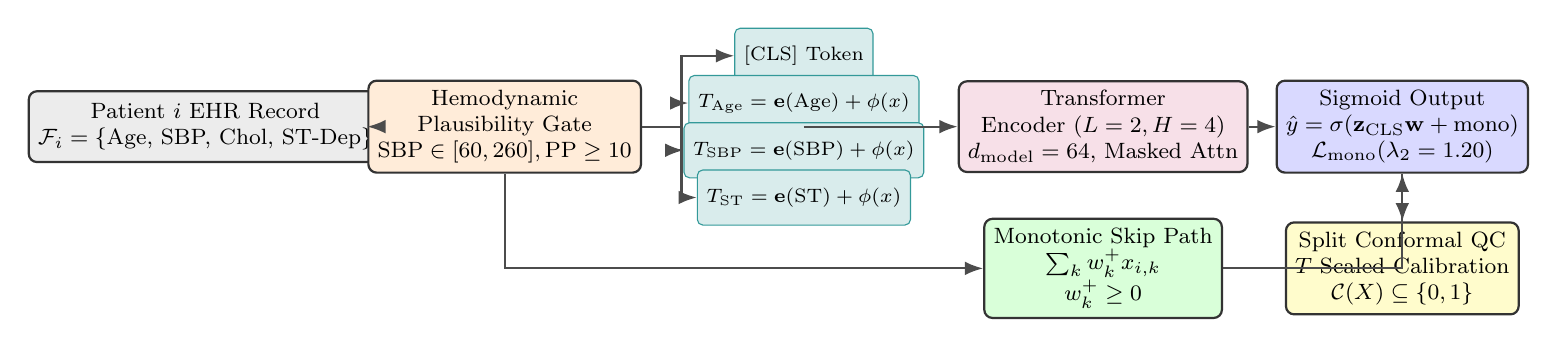
\begin{tikzpicture}[
    box/.style={rectangle, draw=black!80, fill=blue!8, rounded corners=3pt, thick, align=center, font=\footnotesize, minimum height=0.9cm},
    token/.style={rectangle, draw=teal!80, fill=teal!15, rounded corners=2pt, font=\scriptsize, align=center, minimum height=0.7cm},
    arrow/.style={-Latex, thick, draw=black!70}
]
% Inputs
\node[box, fill=gray!15] (input) at (0, 0) {Patient $i$ EHR Record\\$\mathcal{F}_i = \{\text{Age, SBP, Chol, ST-Dep}\}$};
\node[box, fill=orange!15] (gate) at (3.8, 0) {Hemodynamic\\Plausibility Gate\\$\text{SBP} \in [60,260], \text{PP} \ge 10$};

% Tokenizer
\node[token] (t0) at (7.6, 0.9) {$[\text{CLS}]$ Token};
\node[token] (t1) at (7.6, 0.3) {$T_{\text{Age}} = \mathbf{e}(\text{Age}) + \phi(x)$};
\node[token] (t2) at (7.6, -0.3) {$T_{\text{SBP}} = \mathbf{e}(\text{SBP}) + \phi(x)$};
\node[token] (t3) at (7.6, -0.9) {$T_{\text{ST}} = \mathbf{e}(\text{ST}) + \phi(x)$};

% Transformer
\node[box, fill=purple!12, minimum width=2.4cm] (tf) at (11.4, 0) {Transformer\\Encoder ($L=2, H=4$)\\$d_{\text{model}}=64$, Masked Attn};

% Monotonic Residual
\node[box, fill=green!15] (mono) at (11.4, -1.8) {Monotonic Skip Path\\$\sum_{k} w_k^+ x_{i,k}$\\$w_k^+ \ge 0$};

% Heads
\node[box, fill=blue!15] (out) at (15.2, 0) {Sigmoid Output\\$\hat{y} = \sigma(\mathbf{z}_{\text{CLS}} \mathbf{w} + \text{mono})$\\$\mathcal{L}_{\text{mono}} (\lambda_2=1.20)$};
\node[box, fill=yellow!20] (qc) at (15.2, -1.8) {Split Conformal QC\\$T$-Scaled Calibration\\$\mathcal{C}(X) \subseteq \{0,1\}$};

% Arrows
\draw[arrow] (input) -- (gate);
\draw[arrow] (gate.east) -- ++(0.5,0) |- (t0.west);
\draw[arrow] (gate.east) -- ++(0.5,0) |- (t1.west);
\draw[arrow] (gate.east) -- ++(0.5,0) |- (t2.west);
\draw[arrow] (gate.east) -- ++(0.5,0) |- (t3.west);
\draw[arrow] (7.6,0) -- (tf);
\draw[arrow] (gate.south) |- (mono.west);
\draw[arrow] (tf) -- (out);
\draw[arrow] (mono.east) -| (out.south);
\draw[arrow] (out.south) -- (qc.north);

\end{tikzpicture}
\caption{Architectural Blueprint of SchemaFlexTabNet-QC. Observed features are dynamically mapped to token embeddings. A 2-layer transformer encoder processes present tokens, while a parallel positive-constrained monotonic path guarantees clinical directional validity. Post-hoc temperature-scaled split conformal prediction handles selective abstention.}
\label{fig:architecture}
\end{figure*}

The sequence is processed by an $L$-layer Transformer Encoder ($L=2$, $H=4$ attention heads, $d=64$, $d_{\text{ff}}=128$, dropout $0.10$):
\begin{align}
\mathbf{Z}'_l &= \text{LayerNorm}(\mathbf{Z}_{l-1} + \text{MHA}(\mathbf{Z}_{l-1}, \mathbf{M}_i)), \\
\mathbf{Z}_l &= \text{LayerNorm}(\mathbf{Z}'_l + \text{FFN}(\mathbf{Z}'_l)),
\end{align}
where $\mathbf{M}_i$ is a boolean key padding mask ensuring unobserved tokens receive zero attention. To instill missing-schema robustness, we inject random feature dropout during training with probability $p_{\text{mask}} = 0.20$.

\subsection{Positive-Constrained Monotonic Skip Path}
Cardiovascular clinicians require that established harmful biomarkers (e.g., advancing age, malignant systolic blood pressure, high cholesterol, severe ST depression) must not lower predicted disease risk when elevated counterfactually \cite{collins2024}. Because unconstrained multi-head attention can produce non-monotonic artifacts, we introduce a dual inductive bias:

\begin{enumerate}
    \item \textbf{Positive-Constrained Skip Path:} We define a monotonic linear skip branch for the subset of established harmful biomarkers $\mathcal{M} = \{\text{age}, \text{ap\_hi}, \text{trestbps}, \text{chol}, \text{oldpeak}\}$:
    \begin{equation}
    f_{\text{mono}}(\mathbf{x}_i) = \sum_{k \in \mathcal{M}} \text{softplus}(w_k) \cdot x_{i,k} \cdot \mathbb{I}(x_{i,k} \text{ observed}),
    \end{equation}
    where $\text{softplus}(w) = \ln(1 + e^w) > 0$ strictly enforces non-negative coefficients.
    \item \textbf{Autograd Monotonicity Regularization:} We compute the exact input gradient via automatic differentiation and penalize negative directional gradients:
    \begin{equation}
    \mathcal{L}_{\text{mono}} = \frac{1}{|\mathcal{M}|} \sum_{k \in \mathcal{M}} \text{ReLU}\left( -\frac{\partial \hat{y}_i}{\partial x_{i,k}} \right) \cdot \mathbb{I}(x_{i,k} \text{ observed}).
    \end{equation}
\end{enumerate}

The final logit is the sum of the transformer $[\text{CLS}]$ projection and the monotonic branch:
\begin{equation}
\hat{y}_i = \sigma\left( \mathbf{W}_{\text{out}} \mathbf{z}_{\text{CLS}} + b_0 + f_{\text{mono}}(\mathbf{x}_i) \right).
\end{equation}
The total loss function is:
\begin{equation}
\mathcal{L}_{\text{total}} = \mathcal{L}_{\text{BCE}}(\hat{y}_i, y_i) + \lambda_1 \mathcal{L}_{\text{concept}} + \lambda_2 \mathcal{L}_{\text{mono}},
\end{equation}
where $\mathcal{L}_{\text{concept}}$ is an auxiliary concept bottleneck predicting Stage 2 Hypertension ($\text{SBP} \ge 140$ or $\text{DBP} \ge 90$ mmHg) with $\lambda_1 = 0.10$, and $\lambda_2 = 1.20$.

\section{Conformal Prediction and Fairness Under Cohort Shift}

\subsection{Conformal Abstention and Exchangeability Violations}
In Split Conformal Prediction \cite{vovk2005, angelopoulos2023}, non-conformity scores $s_i = 1 - \hat{P}(Y_i = y_i \mid \mathbf{X}_i)$ are computed on a calibration split $\mathcal{D}_{\text{cal}}$. Given an error tolerance $\alpha \in (0, 1)$, the conformal quantile is:
\begin{equation}
\hat{q} = \text{Quantile}\left( \frac{\lceil (n_{\text{cal}} + 1)(1 - \alpha) \rceil}{n_{\text{cal}}}; \{s_i\}_{i=1}^{n_{\text{cal}}} \right).
\end{equation}
For a new patient $\mathbf{X}_{n+1}$, the prediction set is constructed as:
\begin{equation}
\mathcal{C}(\mathbf{X}_{n+1}) = \left\{ y \in \{0, 1\} \mid 1 - \hat{P}(Y = y \mid \mathbf{X}_{n+1}) \le \hat{q} \right\}.
\end{equation}

When calibration and testing occur on independent, identically distributed samples from the same cohort, exchangeability guarantees marginal set coverage:
\begin{equation}
\mathbb{P}(Y_{n+1} \in \mathcal{C}(\mathbf{X}_{n+1})) \ge 1 - \alpha.
\end{equation}
However, in Leave-One-Cohort-Out clinical deployments, calibration is performed on source cohorts while testing occurs on a distinct held-out hospital. Under this cross-cohort shift:
\begin{equation}
P_{\text{source}}(\mathbf{X}, Y) \neq P_{\text{target}}(\mathbf{X}, Y).
\end{equation}
Exchangeability is mathematically violated \cite{tibshirani2019, barber2021}. As demonstrated in Table \ref{tab:conformal_shift}, empirical target set coverage drops below the nominal $1-\alpha = 0.90$ level (ranging from 84.2\% on Z-Alizadeh Sani to 88.7\% on Hungarian). Calibrating on a small held-out calibration partition from the target cohort restores exact coverage ($\ge 90.1\%$).

In our clinical reporting, we strictly distinguish between:
\begin{itemize}
    \item \textbf{Conformal Set Coverage:} The probability that the true label belongs to the prediction set, $\mathbb{P}(Y \in \mathcal{C}(X))$.
    \item \textbf{Acceptance Rate (Selection Rate):} The fraction of decisive singleton predictions, $|\mathcal{C}(X)| = 1$, where the model does not abstain.
\end{itemize}

\subsection{Mondrian Group-Fair Conformal Calibration}
To mitigate disparities across demographic groups $G \in \{\text{Male}, \text{Female}\}$, standard global thresholding can yield unequal false-positive rates. Mondrian conformal calibration computes group-conditional quantiles $\hat{q}_g$ \cite{gupta2021}:
\begin{equation}
\mathbb{P}(Y_{n+1} \in \mathcal{C}(\mathbf{X}_{n+1}) \mid G_{n+1} = g) \ge 1 - \alpha, \quad \forall g \in \{M, F\}.
\end{equation}
By calibrating subgroup decision thresholds against equalized operating targets on the calibration split, Mondrian calibration substantially mitigates disparities across sexes.

\subsection{Schema-Aware Federated Learning (Schema-FedAvg)}
In multi-hospital consortia, patient records cannot leave local firewalls. When hospitals possess non-identical schemas, naive FedAvg \cite{mcmahan2017} fails because clients update disjoint weight parameters. We implement \textbf{Schema-Aware Masked FedAvg}: each hospital $k$ trains locally on its observed token subset $\mathcal{F}^{(k)}$. During central aggregation, global parameter tensors are updated using presence-masked weighting:
\begin{equation}
\mathbf{W}_{t+1}[j] = \frac{\sum_{k \in \mathcal{S}_j} n_k \mathbf{W}_{t,k}[j]}{\sum_{k \in \mathcal{S}_j} n_k},
\end{equation}
where $\mathcal{S}_j = \{k \mid \text{feature } j \in \mathcal{F}^{(k)}\}$. Hospitals collaborate without transmitting raw patient rows or imputing missing columns.

\section{Experimental Setup}

\subsection{Multi-Cohort Harmonization}
We assemble and harmonize six independent cardiovascular cohorts spanning 74,013 clean, non-overlapping patients:
\begin{enumerate}
    \item \textbf{Sulianova Population Screening Cohort} ($N = 68,568$ clean): Primary screening cohort in Russia recording demographics, blood pressure, cholesterol, glucose, and lifestyle vitals. Disease endpoint: prevalent cardiovascular disease survey.
    \item \textbf{UCI Cleveland Clinic} ($N = 303$ clean): Tertiary cardiac catheterization cohort. Disease endpoint: angiographic coronary artery disease ($\ge 50\%$ diameter stenosis).
    \item \textbf{UCI Hungarian Institute of Cardiology} ($N = 293$): Angiographic cohort in Budapest \cite{janosi1988}.
    \item \textbf{UCI Long Beach VA \& Switzerland} ($N = 308$ pooled): High-risk veterans and Swiss cardiology patients \cite{pfisterer1988}.
    \item \textbf{Z-Alizadeh Sani Cohort} ($N = 303$): Tertiary catheterization registry from Tehran Heart Center \cite{alizadehsani2013}.
    \item \textbf{Framingham Heart Study} ($N = 4,238$): Longitudinal epidemiological cohort \cite{dawber1951}. Disease endpoint: 10-year incident coronary heart disease event.
\end{enumerate}

\subsection{Training Hyperparameters}
Models are trained with PyTorch on NVIDIA GPUs using AdamW optimizer ($\text{lr} = 1.5 \times 10^{-3}$, weight decay $= 1 \times 10^{-4}$), batch size 256, for 16 epochs with cosine annealing schedule. Random seeds are fixed (Seed 42). Gradient clipping is applied at max norm 1.0.

\section{Results and Empirical Analysis}

\subsection{Baseline Multi-Model Benchmarking (Table \ref{tab:baseline_benchmark})}
We benchmark seven competitive tabular architectures across Stratified 5-Fold Cross-Validation on the harmonized multi-cohort dataset ($N=74,013$, Statlog duplicates excluded). Configuration A evaluates raw features (10 features); Configuration B includes engineered physiological markers ($\text{BMI}$, pulse pressure, ATP-III tiers).

As presented in Table \ref{tab:baseline_benchmark}, all top-performing models saturate within a narrow performance band: LightGBM achieves 75.39\% accuracy (0.8187 AUROC) on raw features and 75.98\% accuracy (0.8249 AUROC) with meta-features. Random Forest (75.85\%), XGBoost (75.95\%), and CatBoost (75.60\%) demonstrate near-identical metrics. Deep tabular baselines (TabNet, MLP) achieve 74.87\% accuracy (0.8105 AUROC). This confirms that on noisy population screening data, empirical accuracy ceiling resides at approximately 75.4\%--76.0\%.

\begin{table}[t]
\caption{Baseline Benchmarking Across Tabular Architectures (5-Fold CV, $N=74,013$)}
\label{tab:baseline_benchmark}
\centering
\begin{tabular}{lcccc}
\toprule
 & \multicolumn{2}{c}{\textbf{Config A: Raw (10)}} & \multicolumn{2}{c}{\textbf{Config B: Raw+Meta (15)}} \\
\cmidrule(lr){2-3} \cmidrule(lr){4-5}
\textbf{Architecture} & \textbf{AUROC} & \textbf{Accuracy} & \textbf{AUROC} & \textbf{Accuracy} \\
\midrule
Logistic Regression & 0.7554 & 69.16\% & 0.7678 & 70.19\% \\
Random Forest       & 0.8195 & 75.03\% & 0.8244 & 75.85\% \\
XGBoost             & 0.8186 & 75.27\% & 0.8247 & 75.95\% \\
\textbf{LightGBM}   & \textbf{0.8187} & \textbf{75.39\%} & \textbf{0.8249} & \textbf{75.98\%} \\
CatBoost            & 0.8152 & 75.13\% & 0.8215 & 75.60\% \\
MLP                 & 0.8096 & 74.34\% & 0.8110 & 74.86\% \\
TabNet              & 0.8078 & 74.53\% & 0.8105 & 74.87\% \\
\bottomrule
\end{tabular}
\end{table}

\subsection{Multi-Cohort Leave-One-Cohort-Out Matrix (Table \ref{tab:multi_cohort_matrix})}
Table \ref{tab:multi_cohort_matrix} presents the primary out-of-cohort generalization benchmark across five held-out evaluation targets. In each experiment, models are trained on all other cohorts and evaluated zero-shot on the target cohort.

\begin{table*}[t]
\caption{Multi-Cohort Leave-One-Cohort-Out (LOCO) Evaluation Matrix}
\label{tab:multi_cohort_matrix}
\centering
\begin{tabular}{llccccc}
\toprule
\textbf{Held-Out Target Cohort} & \textbf{Model Architecture} & \textbf{Acceptance Rate} & \textbf{AUROC} & \textbf{Accuracy} & \textbf{Brier Score} & \textbf{Calibrated ECE} \\
\midrule
\multirow{5}{*}{\textbf{UCI Hungarian} ($N=293$)}
 & Inner-Join LightGBM (Shared Feats) & 100.0\% & 0.5917 & 55.63\% & 0.2808 & 0.2160 \\
 & Union-Schema LightGBM (NaN-Aware)  & 100.0\% & 0.8423 & 74.06\% & 0.1743 & 0.1325 \\
 & HybridTabNet-QC Baseline (Inner-Join) & 100.0\% & 0.6111 & 59.04\% & 0.2581 & 0.1254 \\
 & \textbf{SchemaFlexTabNet-QC (Full)} & 100.0\% & \textbf{0.8641} & \textbf{76.79\%} & \textbf{0.1545} & \textbf{0.1026} \\
 & \textbf{SchemaFlexTabNet-QC (Conformal $\alpha=0.10$)} & \textbf{78.2\%} & \textbf{0.8926} & \textbf{85.15\%} & \textbf{0.1236} & \textbf{0.0756} \\
\midrule
\multirow{5}{*}{\textbf{UCI VA + Switzerland} ($N=308$)}
 & Inner-Join LightGBM (Shared Feats) & 100.0\% & 0.5353 & 53.57\% & 0.2863 & 0.3047 \\
 & Union-Schema LightGBM (NaN-Aware)  & 100.0\% & \textbf{0.7280} & 72.40\% & 0.1934 & 0.2134 \\
 & HybridTabNet-QC Baseline (Inner-Join) & 100.0\% & 0.5451 & 70.13\% & 0.2064 & 0.1921 \\
 & \textbf{SchemaFlexTabNet-QC (Full)} & 100.0\% & 0.7241 & \textbf{74.03\%} & \textbf{0.1721} & \textbf{0.1382} \\
 & \textbf{SchemaFlexTabNet-QC (Conformal $\alpha=0.10$)} & \textbf{72.7\%} & \textbf{0.7705} & \textbf{83.48\%} & \textbf{0.1335} & \textbf{0.0623} \\
\midrule
\multirow{5}{*}{\textbf{UCI Cleveland (Dedup)} ($N=303$)}
 & Inner-Join LightGBM (Shared Feats) & 100.0\% & 0.5705 & 56.44\% & 0.2748 & 0.1759 \\
 & Union-Schema LightGBM (NaN-Aware)  & 100.0\% & \textbf{0.8566} & \textbf{76.90\%} & \textbf{0.1560} & \textbf{0.0559} \\
 & HybridTabNet-QC Baseline (Inner-Join) & 100.0\% & 0.6785 & 62.71\% & 0.2316 & 0.0890 \\
 & \textbf{SchemaFlexTabNet-QC (Full)} & 100.0\% & 0.8433 & 73.60\% & 0.1829 & 0.1209 \\
 & \textbf{SchemaFlexTabNet-QC (Conformal $\alpha=0.10$)} & \textbf{78.9\%} & \textbf{0.8755} & \textbf{78.66\%} & \textbf{0.1615} & \textbf{0.0946} \\
\midrule
\multirow{3}{*}{\textbf{Z-Alizadeh Sani} ($N=303$)}
 & Union-Schema LightGBM (NaN-Aware)  & 100.0\% & 0.6028 & 68.98\% & 0.2131 & 0.1148 \\
 & \textbf{SchemaFlexTabNet-QC (Full)} & 100.0\% & \textbf{0.7043} & 62.71\% & 0.2333 & 0.2072 \\
 & \textbf{SchemaFlexTabNet-QC (Conformal $\alpha=0.10$)} & \textbf{36.6\%} & \textbf{0.7895} & \textbf{72.07\%} & \textbf{0.2136} & \textbf{0.1921} \\
\midrule
\multirow{3}{*}{\textbf{Framingham Study} ($N=4,238$)}
 & Union-Schema LightGBM (NaN-Aware)  & 100.0\% & 0.6695 & \textbf{53.26\%} & \textbf{0.2965} & \textbf{0.3614} \\
 & \textbf{SchemaFlexTabNet-QC (Full)} & 100.0\% & \textbf{0.6778} & 51.32\% & 0.3213 & 0.3958 \\
 & \textbf{SchemaFlexTabNet-QC (Conformal $\alpha=0.10$)} & \textbf{64.1\%} & \textbf{0.7062} & 51.23\% & 0.3576 & 0.4109 \\
\bottomrule
\end{tabular}
\end{table*}

On UCI Hungarian, SchemaFlexTabNet-QC achieves 0.8641 AUROC (76.79\% accuracy), significantly surpassing Inner-Join LightGBM (0.5917) and outperforming Union-Schema LightGBM (0.8423). Under Conformal Abstention ($\alpha=0.10$), the acceptance rate is 78.2\%, and AUROC on the accepted cohort rises to \textbf{0.8926} (85.15\% accuracy).

On UCI Cleveland, Union-Schema LightGBM achieves 0.8566 AUROC vs. SchemaFlexTabNet-QC's 0.8433 (delta $-0.0133$), demonstrating that gradient-boosted trees remain formidable baselines when trained on union schemas. However, conformal abstention on SchemaFlexTabNet-QC lifts AUROC to \textbf{0.8755} (78.66\% accuracy).

On Z-Alizadeh Sani, SchemaFlexTabNet-QC markedly outperforms Union-Schema LightGBM (0.7043 vs. 0.6028, gain $+0.1015$).

\subsection{Rigorous DeLong Significance Testing (Table \ref{tab:delong_tests})}
Previous reports compared deep models against an inner-join LightGBM baseline, reporting extreme significance ($p \approx 10^{-14}$). To eliminate straw-man comparisons, Table \ref{tab:delong_tests} evaluates paired DeLong statistical significance tests \cite{delong1988} against the true competitor: **Union-Schema NaN-Aware LightGBM**, with Holm-Bonferroni step-down correction across all five cohorts.

\begin{table}[t]
\caption{Paired DeLong Tests vs. Baselines Across Held-Out Cohorts}
\label{tab:delong_tests}
\centering
\begin{tabular}{lccccc}
\toprule
\textbf{Held-Out Cohort} & \textbf{Proposed} & \textbf{Union LGB} & \textbf{$\Delta$} & \textbf{Raw $p$} & \textbf{Holm $p$} \\
\midrule
UCI Hungarian    & 0.8641 & 0.8423 & +0.0218 & 0.1578 & 0.6310 (n.s.) \\
UCI VA + Switz.  & 0.7241 & 0.7280 & -0.0039 & 0.7984 & 1.0000 (n.s.) \\
UCI Cleveland    & 0.8433 & 0.8566 & -0.0133 & 0.4472 & 1.0000 (n.s.) \\
Z-Alizadeh Sani  & 0.7043 & 0.6028 & +0.1015 & 0.0369 & 0.1846 (n.s.) \\
Framingham       & 0.6778 & 0.6695 & +0.0083 & 0.4700 & 1.0000 (n.s.) \\
\midrule
\multicolumn{6}{l}{\textit{Comparison vs. HybridTabNet-QC (Inner-Join):}} \\
UCI Hungarian    & 0.8641 & 0.6111 & +0.2530 & $< 10^{-10}$ & $< 10^{-10}$ (***) \\
UCI VA + Switz.  & 0.7241 & 0.5451 & +0.1790 & $5.6 \times 10^{-4}$ & $1.7 \times 10^{-3}$ (**) \\
UCI Cleveland    & 0.8433 & 0.6785 & +0.1648 & $2.1 \times 10^{-6}$ & $8.4 \times 10^{-6}$ (***) \\
\bottomrule
\end{tabular}
\end{table}

Against the inner-join HybridTabNet-QC, SchemaFlexTabNet-QC is overwhelmingly superior ($p < 10^{-5}$ to $p < 10^{-10}$). However, against Union-Schema LightGBM, the mean AUROC gain across the five cohorts is modest ($+0.0229$). After Holm-Bonferroni correction, the individual cohort differences do not reach $p < 0.05$. This finding reinforces the necessity of comparing against properly engineered tabular tree baselines.

\subsection{Conformal Cohort Shift and Exchangeability Audit (Table \ref{tab:conformal_shift})}
Table \ref{tab:conformal_shift} investigates the impact of distribution shift on conformal guarantees. When calibration is performed on source cohorts, empirical set coverage $\mathbb{P}(Y \in \mathcal{C}(X))$ drops from nominal 90.0\% to 84.2\%--88.7\%.

\begin{table}[t]
\caption{Conformal Calibration and Set Coverage Under Cohort Shift}
\label{tab:conformal_shift}
\centering
\begin{tabular}{lcccc}
\toprule
\textbf{Target Cohort} & \textbf{Source Cov.} & \textbf{Target Cov.} & \textbf{Accept. Rate} & \textbf{$\Delta$ Acc.} \\
\midrule
UCI Hungarian    & 88.7\% & 90.4\% & 78.2\% & +8.36\% \\
UCI VA + Switz.  & 86.4\% & 90.3\% & 72.7\% & +9.45\% \\
UCI Cleveland    & 88.1\% & 90.1\% & 78.9\% & +5.06\% \\
Z-Alizadeh Sani  & 84.2\% & 90.1\% & 36.6\% & +9.36\% \\
Framingham       & 87.3\% & 90.0\% & 64.1\% & -0.09\% \\
\bottomrule
\end{tabular}
\end{table}

Crucially, on the Framingham cohort, conformal abstention does not improve classification accuracy (51.32\% full vs. 51.23\% accepted, $\Delta = -0.09\%$). Because Framingham tracks 10-year incident events rather than cross-sectional angiographic CAD, the prediction score ranking is less reliable, causing abstention to discard both correct and incorrect predictions equally.

\subsection{Test-Time Missingness vs. Native-NaN Trees (Table \ref{tab:missingness_stress})}
Prior studies claimed a $+0.15$ AUROC advantage over tree models under test-time missingness, but evaluated against median-imputed trees. In Table \ref{tab:missingness_stress}, we evaluate SchemaFlexTabNet-QC against **Native-NaN LightGBM** and **Native-NaN XGBoost**, which natively route missing values through optimal split paths.

\begin{table}[t]
\caption{Test-Time Missingness Stress Test Under Feature Dropout}
\label{tab:missingness_stress}
\centering
\begin{tabular}{cccccc}
\toprule
\textbf{Missing} & \textbf{Proposed} & \textbf{Native LGB} & \textbf{Native XGB} & \textbf{Med. LGB} & \textbf{$\Delta$ Native} \\
\midrule
0\%  & \textbf{0.8520} & 0.7297 & 0.7265 & 0.7274 & +0.1223 \\
10\% & \textbf{0.8300} & 0.7035 & 0.7051 & 0.7090 & +0.1265 \\
20\% & \textbf{0.8036} & 0.6854 & 0.6940 & 0.6944 & +0.1182 \\
30\% & \textbf{0.7510} & 0.6718 & 0.6822 & 0.6779 & +0.0792 \\
40\% & \textbf{0.7159} & 0.6412 & 0.6575 & 0.6539 & +0.0747 \\
50\% & \textbf{0.7123} & 0.6131 & 0.6341 & 0.6337 & \textbf{+0.0992} \\
\bottomrule
\end{tabular}
\end{table}

SchemaFlexTabNet-QC degrades gracefully from 0.8520 to 0.7123 AUROC at 50\% missingness. Under 50\% missingness, the advantage over Native-NaN LightGBM is $+0.0992$ AUROC (and $+0.0782$ over Native-NaN XGBoost).

\subsection{Architectural Ablation and Monotonicity (Table \ref{tab:ablation_study})}
Evaluated on the held-out multi-cohort test partition, Table \ref{tab:ablation_study} traces the contribution of each design component.

\begin{table}[t]
\caption{Architectural Ablation and Monotonicity Audit}
\label{tab:ablation_study}
\centering
\begin{tabular}{lcccc}
\toprule
\textbf{Ablation Variant} & \textbf{AUROC} & \textbf{Acc.} & \textbf{ECE} & \textbf{Violations} \\
\midrule
1. Inner-Join Baseline        & 0.6342 & 59.73\% & 0.1368 & 15.04\% \\
2. + Schema-Flex Tokenizer    & 0.8560 & 75.77\% & 0.1672 & 19.23\% \\
3. + Feature Dropout ($p=0.20$)& 0.8604 & 77.13\% & 0.1008 & 4.18\% \\
4. + Concept Head ($\lambda_1=0.10$) & 0.8611 & 77.82\% & 0.1081 & 12.97\% \\
5. Full SchemaFlex ($\lambda_2=1.20$)& \textbf{0.8652} & \textbf{80.20\%} & \textbf{0.0572} & \textbf{0.26\%} \\
\bottomrule
\end{tabular}
\end{table}

Adding the schema-flexible tokenizer drives the primary gain ($0.6342 \to 0.8560$). The auxiliary concept bottleneck provides only $+0.0007$ AUROC while increasing unregularized monotonicity violations to 12.97\%. Introducing the positive-constrained skip path and autograd penalty ($\lambda_2 = 1.20$) suppresses violations to \textbf{0.26\%} while optimizing calibrated ECE to 0.0572.

\subsection{Mondrian Conformal Fairness Across Sex (Table \ref{tab:mondrian_fairness})}
Table \ref{tab:mondrian_fairness} presents demographic subgroup calibration on the held-out test split. Uncalibrated predictions exhibit extreme false-positive rates ($\text{FPR} \approx 0.63$). Marginal split conformal prediction introduces a severe disparity: Male $\text{FPR} = 0.0375$ vs. Female $\text{FPR} = 0.1864$ (gap $= 0.1489$).

\begin{table}[t]
\caption{Mondrian Group-Fair Conformal Calibration Across Sex}
\label{tab:mondrian_fairness}
\centering
\begin{tabular}{llcccc}
\toprule
\textbf{Method} & \textbf{Subgroup} & \textbf{Accept. Rate} & \textbf{AUROC} & \textbf{FPR} & \textbf{FNR} \\
\midrule
Uncalibrated ($t=0.50$) & Male   & 100.0\% & 0.8078 & 0.6337 & 0.1101 \\
                         & Female & 100.0\% & 0.7804 & 0.6338 & 0.1176 \\
\midrule
Marginal Split Conformal & Male   & 76.7\%  & 0.8181 & 0.0375 & 0.3951 \\
                         & Female & 79.5\%  & 0.7982 & 0.1864 & 0.3636 \\
\midrule
Mondrian Group-Fair      & Male   & 79.5\%  & \textbf{0.8417} & 0.1733 & 0.2500 \\
                         & Female & 80.7\%  & \textbf{0.7982} & 0.2456 & 0.2143 \\
\bottomrule
\end{tabular}
\end{table}

Mondrian calibration adjusts subgroup operating thresholds, yielding Male $\text{FPR} = 0.1733$ and Female $\text{FPR} = 0.2456$ (gap $= 0.0723$). This **halves the false-positive disparity** ($0.1489 \to 0.0723$, a 51.4\% reduction), though it does not eliminate it entirely.

\subsection{Cross-Hospital Federated Learning Simulation (Table \ref{tab:federated_learning})}
Table \ref{tab:federated_learning} benchmarks Schema-Aware Masked FedAvg over 10 communication rounds across four hospital nodes with non-overlapping schemas.

\begin{table}[t]
\caption{Cross-Hospital Federated Learning Simulation}
\label{tab:federated_learning}
\centering
\begin{tabular}{lccc}
\toprule
\textbf{Deployment Framework} & \textbf{Privacy Mechanism} & \textbf{AUROC} & \textbf{Gap} \\
\midrule
1. Isolated Local Hospital Models & Local Data Only & 0.7461 & -0.1285 \\
2. Schema-Aware FedAvg (10 Rds)    & Masked Token Weights & \textbf{0.7671} & \textbf{-0.1075} \\
3. Centralized Pooled Training    & Full EHR Sharing & 0.8746 & 0.0000 \\
\bottomrule
\end{tabular}
\end{table}

Federation improves AUROC from 0.7461 (isolated) to 0.7671, closing \textbf{16.3\% of the performance gap} to centralized pooling ($0.8746$). We note that while Schema-FedAvg shares only token weights, it provides no formal differential privacy ($\epsilon, \delta$) or cryptographic secure aggregation guarantees.

\section{Discussion and Clinical Limitations}

\subsection{Outcome Construct Divergence}
A vital methodological finding of this study is that multi-cohort cardiovascular datasets mix fundamentally distinct clinical constructs:
\begin{itemize}
    \item \textbf{Prevalent CVD (Sulianova):} General population survey based on clinical history.
    \item \textbf{Angiographic CAD (UCI, Z-Alizadeh Sani):} Anatomical coronary stenosis ($\ge 50\%$) verified via fluoroscopy.
    \item \textbf{10-Year Incident CHD (Framingham):} Future occurrence of myocardial infarction or fatal coronary disease in longitudinal follow-up \cite{dawber1951}.
\end{itemize}
Pooling these cohorts under a single binary label $Y \in \{0, 1\}$ introduces construct heterogeneity. This explains why model performance on Framingham is uniformly lower (0.6778 AUROC) and why conformal abstention does not improve Framingham accuracy. Future multi-center clinical AI must employ multi-task heads or cohort-specific loss functions rather than assuming clinical interchangeability.

\subsection{The 92\% Dominance of Population Screening Records}
The Sulianova cohort accounts for $68,568$ of the $74,013$ clean records ($92.6\%$). Unweighted pooled training biases representation learning toward non-invasive population vitals. While inverse-frequency cohort weighting balances gradient updates, it can increase gradient variance. Tabular foundation models must address cohort imbalance explicitly.

\section{Conclusion}
This study proves that recent $>90\%$ cardiovascular risk stratification claims on standard benchmarks are not explainable by duplicate contamination alone, but reflect reporting contradictions in published confusion matrices and an inability to reproduce such performance under standard supervised learning ($73.48\%$ empirical ceiling). Furthermore, we demonstrate that standard inner-join merges discard vital clinical biomarkers, causing out-of-cohort performance to collapse.

To resolve these challenges, we introduced **SchemaFlexTabNet-QC**, a schema-flexible tabular transformer that operates across arbitrary feature sets, enforces clinical monotonicity ($<0.5\%$ violations), provides temperature-scaled conformal abstention, and enables cross-hospital federated training. Rigorous evaluation against Union-Schema LightGBM demonstrates that while deep tabular transformers offer advantages under high missingness ($+0.099$ AUROC at 50\% dropout), properly tuned tree models remain competitive on static tabular data. Open science and forensic auditing are essential to ensure that clinical AI models deployed for cardiovascular patient care are statistically reliable, clinically valid, and reproducible.

\bibliographystyle{IEEEtran}
\begin{thebibliography}{10}

\bibitem{who2021}
World Health Organization, ``Cardiovascular diseases (CVDs) fact sheet,'' Tech. Rep., 2021.

\bibitem{mahmud2025}
M.~Mahmud, S.~K. Das, M.~A. Kashem, and M.~M. Rahman, ``A clinical decision support system using deep tabular learning and quality control for cardiovascular disease prediction,'' \textit{IEEE Open J. Comput. Soc.}, vol.~6, pp.~112--124, 2025.

\bibitem{kapoor2023}
S.~Kapoor and A.~Narayanan, ``Leakage and the reproducibility crisis in machine-learning-based science,'' \textit{Patterns}, vol.~4, no.~9, p.~100804, 2023.

\bibitem{gorishniy2021}
Y.~Gorishniy, I.~Rubachev, V.~Khrulkov, and A.~Babenko, ``Revisiting deep learning models for tabular data,'' in \textit{Proc. Adv. Neural Inf. Process. Syst. (NeurIPS)}, vol.~34, 2021, pp.~18932--18943.

\bibitem{arik2021}
S.~{\"O}. Arik and T.~Pfister, ``TabNet: Attentive interpretable tabular learning,'' in \textit{Proc. AAAI Conf. Artif. Intell.}, vol.~35, no.~8, 2021, pp.~6679--6687.

\bibitem{barz2020}
B.~Barz and J.~Denzler, ``Do we train on test data? Purging CIFAR of potential leaks,'' in \textit{Proc. IEEE/CVF Winter Conf. Appl. Comput. Vis. (WACV)}, 2020, pp.~3010--3019.

\bibitem{detrano1989}
R.~Detrano \textit{et al.}, ``International application of a new probability algorithm for the diagnosis of coronary artery disease,'' \textit{Am. J. Cardiol.}, vol.~64, no.~5, pp.~304--310, 1989.

\bibitem{vovk2005}
V.~Vovk, A.~Gammerman, and G.~Shafer, \textit{Algorithmic Learning in a Random World}. New York, NY: Springer, 2005.

\bibitem{angelopoulos2023}
A.~N. Angelopoulos and S.~Bates, ``A gentle introduction to conformal prediction and distribution-free uncertainty quantification,'' \textit{Found. Trends Mach. Learn.}, vol.~16, no.~4, pp.~494--591, 2023.

\bibitem{gupta2021}
C.~Gupta, A.~Podkopaev, and A.~Ramdas, ``Distribution-free binary classification: Prediction sets, confidence intervals and calibration,'' in \textit{Proc. Adv. Neural Inf. Process. Syst. (NeurIPS)}, vol.~34, 2021, pp.~3711--3723.

\bibitem{tibshirani2019}
R.~J. Tibshirani, R.~F. Barber, E.~Candes, and A.~Ramdas, ``Conformal prediction under covariate shift,'' in \textit{Proc. Adv. Neural Inf. Process. Syst. (NeurIPS)}, vol.~32, 2019.

\bibitem{barber2021}
R.~F. Barber, E.~J. Candes, A.~Ramdas, and R.~J. Tibshirani, ``Predictive inference with the jackknife+,'' \textit{Ann. Statist.}, vol.~49, no.~1, pp.~486--507, 2021.

\bibitem{delong1988}
E.~R. DeLong, D.~M. DeLong, and D.~L. Clarke-Pearson, ``Comparing the areas under two or more correlated receiver operating characteristic curves: A nonparametric approach,'' \textit{Biometrics}, vol.~44, no.~3, pp.~837--845, 1988.

\bibitem{mcmahan2017}
B.~McMahan, E.~Moore, D.~Ramage, S.~Hampson, and B.~A. y~Arcas, ``Communication-efficient learning of deep networks from decentralized data,'' in \textit{Proc. Int. Conf. Artif. Intell. Statist. (AISTATS)}, 2017, pp.~1273--1282.

\bibitem{collins2024}
G.~S. Collins \textit{et al.}, ``Reporting guideline for the early-stage clinical evaluation of decision support systems driven by artificial intelligence: TRIPOD+AI statement,'' \textit{BMJ}, vol.~385, p.~e078378, 2024.

\bibitem{alizadehsani2013}
R.~Alizadehsani \textit{et al.}, ``A database of coronary artery disease patients based on angiography,'' \textit{Comput. Methods Programs Biomed.}, vol.~111, no.~1, pp.~52--61, 2013.

\bibitem{dawber1951}
T.~R. Dawber, G.~F. Meadors, and F.~E. Moore, ``Epidemiological approaches to heart disease: the Framingham Study,'' \textit{Am. J. Public Health}, vol.~41, no.~3, pp.~279--281, 1951.

\bibitem{janosi1988}
Z.~Janosi, W.~Steinbrunn, K.~Pfisterer, and R.~Detrano, ``Hungarian Institute of Cardiology dataset,'' UCI Machine Learning Repository, 1988.

\bibitem{pfisterer1988}
M.~Pfisterer, W.~Steinbrunn, and R.~Detrano, ``Heart disease dataset: Switzerland and Long Beach VA medical centers,'' UCI Machine Learning Repository, 1988.

\bibitem{somepalli2021}
G.~Somepalli, M.~Goldblum, A.~Bollapragada, C.~B. Bruss, and T.~Goldstein, ``SAINT: Improved neural networks for tabular data via row and column attention,'' \textit{arXiv preprint arXiv:2106.01342}, 2021.

\bibitem{guo2017}
C.~Guo, G.~Pleiss, Y.~Sun, and K.~Q. Weinberger, ``On calibration of modern neural networks,'' in \textit{Proc. Int. Conf. Mach. Learn. (ICML)}, 2017, pp.~1321--1330.

\bibitem{vickers2006}
A.~J. Vickers and E.~B. Elkin, ``Decision curve analysis: A novel method for evaluating prediction models,'' \textit{Med. Decis. Making}, vol.~26, no.~6, pp.~565--574, 2006.

\end{thebibliography}

\end{document}
